\documentclass{book}
\usepackage{graphicx}
\usepackage{color}
\usepackage{url}
\usepackage{fontspec}	% To change default font
\usepackage{fancyhdr}	%to include customized footer and header
\pagestyle{fancy}
\lhead{}
\chead{\leftmark}
\graphicspath{{./Figures/}}
\setmainfont{URW Palladio L} % Use if font is to be set

\begin{document}
%-----------------------------------
% For customised Title Page
\thispagestyle{empty}
%\input{./title.tex} %Cover page
\thispagestyle{empty}
%\input{./inner.tex}	%Inner title page
%--------------------------------------------------------------------

%Default Title page 
\title{Analog Communication
Laboratory Manual}
\date{December 2013}
%\author { Kavya Manohar}
\maketitle
%----------------------------------------------------------
%\thispagestyle{empty}
  
\textcopyright{}2013 
\\[10cm]
    
%------------------------------------------------------------






\thispagestyle{empty}
\tableofcontents
\thispagestyle{empty}
\thispagestyle{empty}

\listoffigures
\thispagestyle{empty}

\chapter [Introduction to Analog Communication]{Introduction to Analog Communication}


\cite{ACmanual}Communication is the transfer of information from one place to another. A bidirectional communication system operates in opposite directions. The receiver can respond
to the sender. Radio communication uses electrical energy to transmit information. Because electrical energy travels almost as fast as light, radio communication is essentially instantaneous.
A radio transmitter converts audio (sound) signals to electrical signals that are sent over wires or through space. A radio receiver converts the electromagnetic waves back to sound waves so that the
information can be understood. 

The transmitted information is the \textbf {intelligence signal} or \textbf{ message signal}.
 Message signals are in the \textbf {Audio Frequency (AF)} range of low frequencies from about 20 Hz to 20 kHz.
 
 
The \textbf{Radio Frequency (RF)}  is the carrier signal. Carrier signals have high frequencies that range from 10 kHz up to about 1000 GHz.
A radio transmitter sends the low frequency message signal at the higher carrier signal frequency by combining the message signal with the carrier signal.

\textbf{Modulation} is the process of changing a characteristic of the carrier signal with the message
signal. In the transmitter, the message signal modulates the carrier signal.
The modulated carrier signal is sent to the receiver where \textbf{demodulation} of the carrier occurs to
recover the message signal.\\[10pt]
\textsc{\textbf {IMPORTANT TERMS}}
\begin{itemize}
\item \textbf{Audio} - signals that a person can hear.

\item \textbf{Electromagnetic waves} - the radiant energy produced by oscillation of an electric
charge.

\item \textbf{Intelligence signal} - any signal that contains information; it is also called the
message signal.
\item \textbf{Message signal} - any signal that contains information; it is also called
the intelligence signal. 
\item \textbf{Audio Frequency (AF)} - frequencies that a person can hear.
AF signals range from about 20 Hz to 20 kHz.
\item \textbf{Radio Frequency (RF)} - the transmission frequency of electromagnetic (radio) signals.
RF frequencies are from about 300 kHz to the 1,000,000 kHz range.
\item \textbf{Carrier signal} - a single, high-frequency signal that can be modulated by a message
signal and transmitted.
\item \textbf{Modulation} - the process of combining the message signal with the carrier signal that
causes the message signal to vary a characteristic of the carrier signal.
\item \textbf{Demodulation} - the process of recovering or detecting the message signal from the
modulated carrier frequency.
\item \textbf{Amplitude Modulation (AM)} - the process of combining the message signal with
the carrier signal and the two sidebands: the lower sideband and the upper
sideband.
\item \textbf{Frequency Modulation (FM)} - the process of combining the message signal with
the carrier signal that causes the message signal to vary the frequency of the
carrier signal.
\item \textbf{Phase Modulation (PM)} - the process of combining the message signal with the
carrier signal that causes the message signal to vary the phase of the carrier signal.
\item \textbf{Angle modulation} - the process of combining the message signal with the carrier signal that causes the message signal to vary the frequency and/or phase of the
carrier signal.
\item \textbf{Balanced modulator} - an amplitude modulator that can be adjusted to control the
amount of modulation.
\item \textbf{Double-Sideband (DSB)} - an amplitude modulated signal in which the carrier is
suppressed, leaving only the two sidebands: the lower sideband and the upper
sideband.
\item \textbf{Mixer}- an electronic circuit that combines two frequencies.
\item \textbf{Product detector} - a detector whose audio frequency output is equal to the product of the
Beat
Frequency Oscillator (BFO) and the RF signal inputs.
\item \textbf{Phase detector} - an electronic circuit whose output varies with the phase differential
of the two input signals.
\item \textbf{Envelopes}- the waveform of the amplitude variations of an amplitude modulated
signal. 
\item \textbf{Sidebands} - the frequency bands on each side of the carrier frequency that
are formed during modulation; the sideband frequencies contain the intelligence of
the message signal.
\item \textbf{AM} - an amplitude modulated signal that contains the carrier signal and the two
sidebands: the lower sideband and the upper sideband.
\item \textbf{Bandwidth} - the frequency range, in hertz (Hz), between the upper and lower
frequency limits. 
\item \textbf{Harmonics} - signals with frequencies that are an integral multiple of
the fundamental frequency. 
\item \textbf{Beat Frequency Oscillator (BFO)} - an oscillator whose
output frequency is approximately equal to the transmitter's carrier frequency and is
input to a product detector
\end {itemize}
\chapter[Amplitude Modulation- Generation]{Amplitude Modulation- Generation}

\section*{Aim}
To design and set-up  an AM generator using BJT and measure the modulation index from the observed output waveform.

\section*{Theory}
\paragraph{}
	The transistor $T_1$ is configured as a common emitter amplifier. The RF carrier wave is given at the base through a coupling capacitor $C_1$.  The message signal used for modulation is the AF signal applied between the emitter resistance and the ground. The message signal modulates the envelope of the carrier which is obtained as output from the collector through a coupling capacitor $C_3$. 
\paragraph{}
The ratio of the maximum amplitude of the modulating signal voltage to that of the carrier voltage is termed as modulation index. This is represented as $m=\frac{V_m}{V_c}$.


\section*{Design}
\textcolor{red}{Design steps need to be verified}
\paragraph{}
Choose BF194 which is a high frequency transistor. From its datasheet the various parameters can be obtained as:

  Type Designator: BF194

Material of transistor: Si

Polarity: NPN

Maximum collector power dissipation ($Pc$), W: 0.25

Maximum collector-base voltage |$V_{cb}$|, V: 30

Maximum collector-emitter voltage |$V_{ce}$|, V: 20

Maximum emitter-base voltage |$V_{eb}$|, V: 5

Maximum collector current |$I_{c max}$|, mA: 30

Forward current transfer ratio (hFE), min: 67

\paragraph{DC Biasing conditions:}

  Let the supply voltage be 60\% of the maximum $V_{ce}$.  \begin{equation}
V_{cc}=\ 60\% of V_{cemax}=\ 12 V
\end{equation}

\noindent Let the collector current $I_c$ be 10\% of maximum rated value.
\begin{equation}
I_{c}=\ 3\% \ of \ I_{cmax}=\ 1 mA
\end{equation}

\noindent In-order to fix the biasing point in the middle of load line, let $V_{RC}$ be 40\% of $V_{cc}$, $V_{RE}$\ be\ 10\% \ of $V_{cc}$ and $V_{ce}$\  be\ 50\% \ of $V_{cc}$.
\begin{equation}
V_{RC}=\ 45\% \ of \ V_{cc}=\ 5.4V
\end{equation}
\begin{equation}
V_{RE}=\ 5\% \ of \ V_{cc}=\ 0.6V
\end{equation}
\begin{equation}
V_{ce}=\ 50\% \ of \ V_{cc}=\ 6V
\end{equation}
\paragraph{Design of Resistors:}
\begin{equation}
R_C=\frac{V_{RC}}{I_c}=\ \frac{5.4V}{1mA}=\ 5.4 k\Omega
\end{equation}
\begin{equation}
R_E=\frac{V_{RE}}{I_e}=\ \frac{0.6V}{1mA}=\ 600\Omega
\end{equation}
\noindent From the datasheet, hFE has a minium value of 67. 
\begin{equation}
I_b=\frac{I_c}{hFE}=\frac{1mA}{67}=\ 15 \mu A
\end{equation}
\noindent Assume the current through $R_1=\ 10 I_b$ and that through $R_2=9I_b$ 
\begin{equation}
 V_{R2}=V_{be}+V_{RE}\\ =0.7+0.6V=1.3V
\end{equation}
\noindent Then
\begin{equation}
R_2=\frac{V_{R2}}{9I_b}=\frac{1.2V}{9X15X10^{-6}}=8.8 k\Omega
\end{equation}
\noindent and 
\begin{equation}
R_1=\frac{V_{R1}}{10I_b}=\frac{10.8V}{10X15X10{^-6}}= 72k\Omega
\end{equation}

\noindent Based on these design equations use the standard resistor values of $R_1=22k\Omega,\ R_2=10k\Omega, \ R_c=10k\Omega,\ R_c=560\Omega$ and a load resistance of $R_L=1k\Omega$.
Use coupling capacitors $C_1=0.1 \mu F,\ C_2=0.001\mu F$ and emitter bye-pass capacitor $C_E=0.01\mu F$.
\subsection*{Components and Equipments Required}
Function Generators(2), CRO(2), Connection wires, Probes.
\\BF194 - High frequency bipolar junction transistor
\\ $22k\Omega,\  10k\Omega\ (2),\ 560\Omega,\,\ 1k\Omega $ - Resistors
\\ $ 0.1\mu F,\ 0.01\mu F, \ 0.001\mu F $ - Capacitors
\\ 
\section*{Circuit Diagram}
\begin{figure}[h]
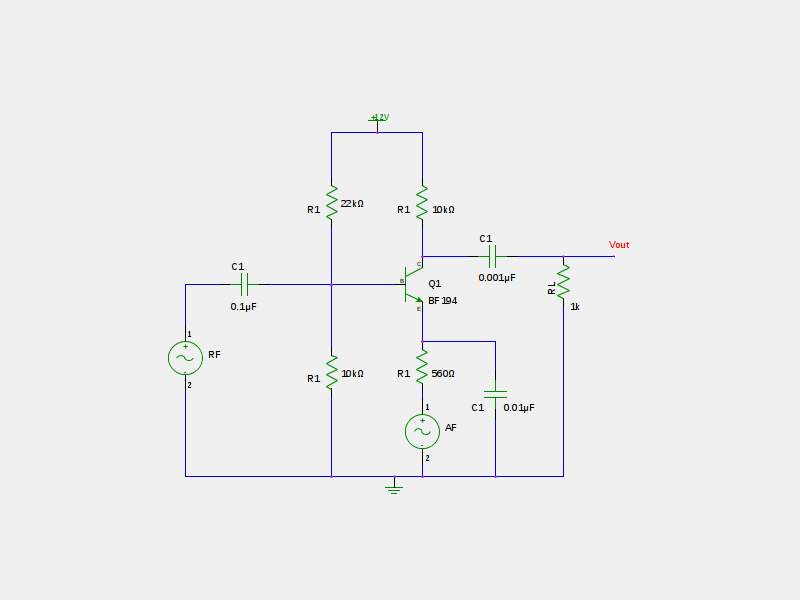
\includegraphics[width=15cm, height=10cm, trim=5cm 3.5cm 4cm 3.5cm, clip=true]{AM.png}
\caption{Circuit Diagram for Amplitude modulation using BJT}

\end{figure}

\section*{Procedure}
\begin{enumerate}
\item
Set up the circuit after verifying the condition of components.
\item
Feed AF modulating signal (say, $f_m=1kHz$ and $E_m=150mV$) and Rf carrier (say, $f_c=70kHz$ and $E_c=300mV$) using function generators.
\item
Adjust amplitude and frequencies of the AF and RF signals and observe amplitude modulated waveform on the CRO.
\item
Fix $f_m$ and $f_c$. Note down $E_{max}$ and $E_{min}$ of the AM signal and calculate modulation index according to the formula 
\begin{equation}
m=\frac{E_{max}-E_{min}}{E_{max}+E_{min}}
\end{equation}
\item
Repeat for different values of $E_m$ and $E_c$. Observe the AM waveforms for different values of m.
\item
Plot the waveforms on a graph sheet.
\item

Fill in the observation column
\end{enumerate}


\section*{Observation}

\begin{figure}[h]
\label{AMmodindex}
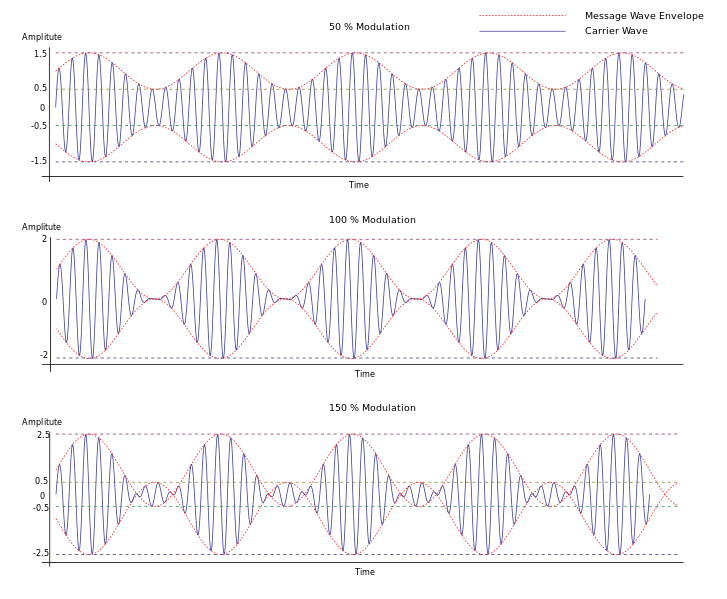
\includegraphics[width=\textwidth]{AMmodindex.png}
\caption{Effect of modulation index on AM}
\end{figure}
\noindent Fig .\ref{AMmodindex}  shows the effect of modulation index on the resultant AM wave\footnote{\url{https://commons.wikimedia.org:/wiki/File:Amplitude_Modulated_Wave-hm-64.svg}}
\begin{center}

\begin{tabular}{|l|l|l|}

\hline
$E_{min}$  & $E_{max}$ & $m=\frac{E_{max}-E_{min}}{E_{max}+E_{min}}$ \\
 & & \\ \hline
 & & \\ \hline
& & \\ \hline
& & \\ \hline
& & \\ \hline
& & \\ \hline

\end{tabular}
\end{center}


\section*{Result}

Implemented the AM modulation circuit using BJT.
The modulation index corresponding to $E_m=$ \textemdash \textemdash and $E_c=$ \textemdash\textemdash is : m= \textemdash\textemdash .






\chapter[Amplitude Modulation - Detection]{Amplitude Modulation - Detection}
\chapter[Intermediate Frequency Amplifier]{Intermediate Fequency Amplifier}

\chapter[Mixer Circuit using FET and BJT]{Mixer Circuit using FET and BJT}

\chapter[Balanced Modulator for DSB-SC]{Balanced Modulator for DSB-SC}



\chapter[FM generation - Reactance Modulator]{FM generation - Reactance Modulator}

\chapter[FM Demodulation]{FM Demodulation}

\chapter[PAM Generation and Demodulation]{PAM Generation and Demodulation}

\chapter[Intermediate Fequency Amplifier]{Intermediate Fequency Amplifier}

\chapter[FM Demodulation using PLL]{FM Demodulation using PLL}

\chapter[AM generation and Demodulation]{AM generation and Demodulation}

\chapter[SSB generation and Demodulation]{SSB generation and Demodulation}

\begin{thebibliography}{1}
\bibitem{ACmanual}{LABORATORY MANUAL COMMUNICATIONS LABORATORYEE 321, CALIFORNIA STATE UNIVERSITY, LOS ANGELES
Lab-Volt Systems, Inc}

\end{thebibliography}


\end{document}
